\documentclass[tikz,border=2]{standalone}
\usetikzlibrary{shadows,arrows,shapes,positioning,calc,backgrounds,fit}
% Define the layers to draw the diagram
%
\begin{document}
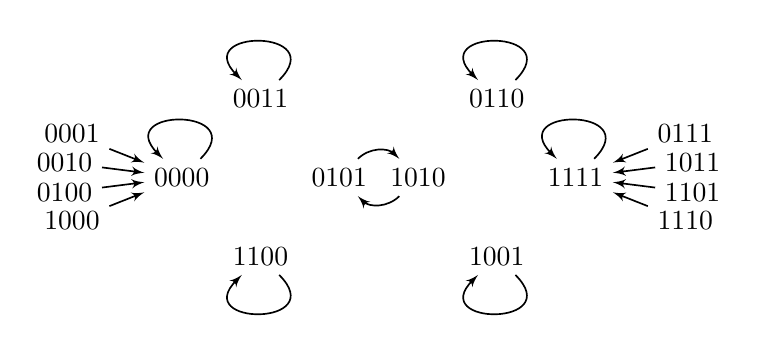
\begin{tikzpicture}
[node distance=1cm,
every node/.style={draw=none},
edge/.style={->,>=latex', shorten >=.0pt, shorten <=.0pt, semithick}]
%%
\begin{scope}[shift={(0,0)}]
\node (0000) at (0,0) {$0000$} edge[loop,edge,out=45,in=135,looseness=5] (0000);
%%
\def \n {10}
\def \rad {1.5cm}
\node (0001) at ({360/\n * 4.4}:\rad) {$0001$};
\node (0010) at ({360/\n * 4.8}:\rad) {$0010$};
\node (0100) at ({360/\n * 5.2}:\rad) {$0100$};
\node (1000) at ({360/\n * 5.6}:\rad) {$1000$};
%%
\draw[edge] (0001) -- (0000);
\draw[edge] (0010) -- (0000);
\draw[edge] (0100) -- (0000);
\draw[edge] (1000) -- (0000);
\end{scope}
%%
%%
\begin{scope}[shift={(5,0)}]
\node (1111) at (0,0) {$1111$} edge[loop,edge,out=45,in=135,looseness=5] (1111);
%%
\def \n {10}
\def \rad {1.5cm}
\node (0111) at ({360/\n * 0.6}:\rad) {$0111$};
\node (1011) at ({360/\n * 0.2}:\rad) {$1011$};
\node (1101) at ({360/\n * -0.2}:\rad) {$1101$};
\node (1110) at ({360/\n * -0.6}:\rad) {$1110$};
%%
\draw[edge] (0111) -- (1111);
\draw[edge] (1011) -- (1111);
\draw[edge] (1101) -- (1111);
\draw[edge] (1110) -- (1111);
\end{scope}
%%
%%
\begin{scope}[shift={(2.5,0)}]
\node (0101) at (-.5,0) {$0101$};
\node (1010) at (.5,0) {$1010$};
\draw[edge] (0101) [out=45,in=135] to (1010);
\draw[edge] (1010) [out=-135,in=-45] to (0101);
\end{scope}
%%
\node (0011) at (1,1) {$0011$} edge[loop,edge,out=45,in=135,looseness=5] (0011);
\node (0110) at (4,1) {$0110$} edge[loop,edge,out=45,in=135,looseness=5] (0110);
\node (1100) at (1,-1) {$1100$} edge[loop,edge,out=-45,in=-135,looseness=5] (1100);
\node (1001) at (4,-1) {$1001$} edge[loop left,edge,out=-45,in=-135,looseness=5] (1001);
%%
%%\draw[edge] (0011) edge[loop,out=45,in=90] (0011);
\end{tikzpicture}
\end{document}

